\documentclass{article}
\usepackage[utf8]{inputenc}
\usepackage{amsmath}
\usepackage{amsthm}
\usepackage{amssymb}
\usepackage{amsfonts}
\usepackage{mathtools}
\usepackage{hyperref}
\usepackage{float}
\usepackage{bm}
\usepackage{comment}
\date{}
\usepackage[margin=0.5in]{geometry}
\begin{document}
\section{Synthetic Experiments}
\subsection{O(5) Invariant Task} 
A synthetic O(5) invariant regression problem given by the function
\begin{align}f(x_1,x_2) = \sin(\Vert x_1\Vert)-\frac{\Vert x_2\Vert^3}{2}+\frac{x_1^\top x_2}{\Vert x_1\Vert\Vert x_2\Vert}, \quad x_1,x_2\in\mathbb{R}^5.
\end{align}

We train a neural network to find a function $g(\cdot)$ such that:
\begin{align}
    f(x_1,x_2) = g(x_1^\top x_1, x_1^\top x_2, x_2^\top x_2).
\end{align}
See results in Figure \ref{fig:O5invariant}.
\begin{figure}[H]
   \centering
   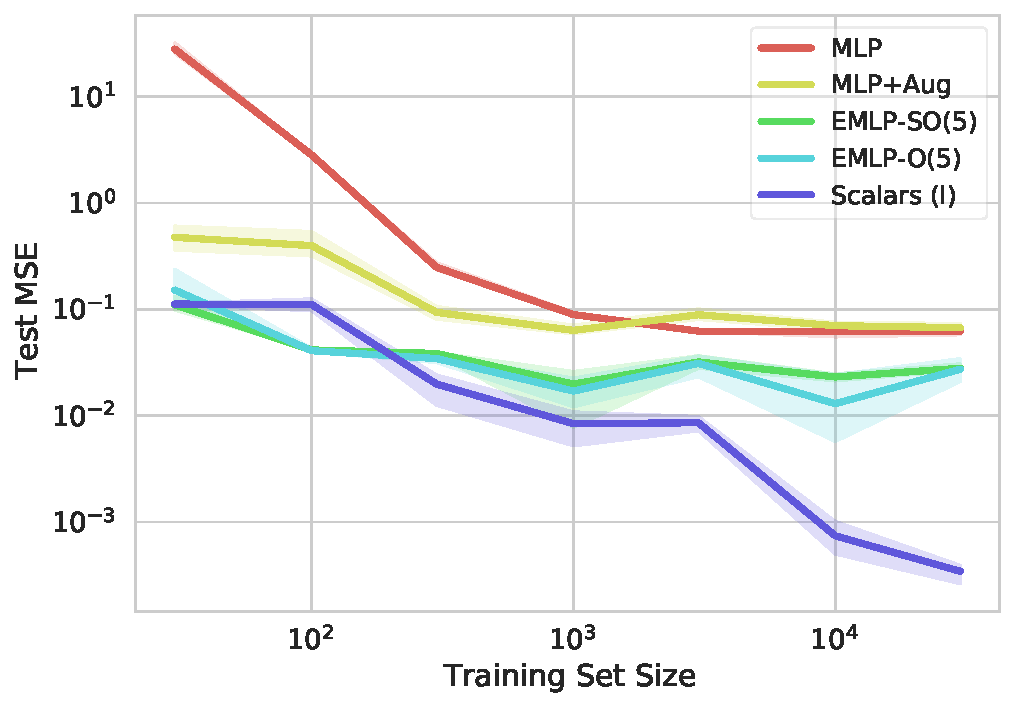
\includegraphics[scale=0.45]{data_efficiency_O5Synthetic.pdf}
   \caption{O(5) invariant task.}
   \label{fig:O5invariant}
\end{figure}

\subsection{O(3) Equivariant Task}
Predicting the moment of inertia matrix from $n=5$ point masses and positions $\{(m_i,x_i)\}_{i=1}^5$,
\begin{align}
\mathcal{I} =\sum_{i=1}^5 m_i(x_i^\top x_i I- x_ix_i^\top), \quad m_i\in\mathbb{R},x_i\in \mathbb{R}^5,i=1,2,\ldots,5.
\end{align}
The inputs $X = \{(m_i,x_i)\}_{i=1}^5$ are of type $5T_0+5T_1$ and outputs are of type $T_2$, both transform under the group.


\paragraph{O(d)-equivariant formulation} See Proposition 4. Denote the set of $3\times 3$ matrices $\mathcal{M} = \{x_ix_j^\top, \forall i,j\}\cup{I}$ (identity matrix). The idea is to approximate the following
\begin{align}
    \sum_{M\in\mathcal{M}}f_{M}\big(x_1^\top x_1,x_1^\top x_2, \ldots, x_4^\top x_5, x_5^\top x_5, m_1,m_2,\ldots,m_5\big)\; M,
\end{align}
where each corresponding $f_{M}$ is some multi-layer perceptron. See \texttt{Scalars (E)} in Figure \ref{fig:O3equivariant}.
\paragraph{O(d)-equivariant $+$ permutation invariant formulation}
See Proposition 10. 
The general idea is to approximate the sum of values of the two functions 
\begin{align}
    \sum_{i,j}f_{ij}(\{x_i^\top x_j, m_i,m_j\}, \{x_k^\top x_l,m_k, m_l,\forall k,l\})\; x_ix_j^\top 
\end{align}
and 
\begin{align}
    f_0(\{x_i^\top x_j, m_i,m_j, \forall i,j\}) I,
\end{align}
where $f_{ij}$ and $f_0$ can be some multi-layer perceptrons. 
For example, we can apply a function on $x_ix_j^\top$ for all pairs of particles $(i,j)$, $i\neq j$, and another function on $x_ix_i^\top$ for all $i$. To be more specific, 
\begin{align}
    \sum_{i\neq j} f_1\big(x_i^\top x_j, \theta_1(m_i)+\theta_1(m_j), \sum_{k,l}\phi_1(x_k^\top x_l), \sum_s\psi_1(m_s)\big) x_ix_j^\top
\end{align}

\begin{align}
    \sum_{i} f_2\big(x_i^\top x_i, \theta_2(m_i), \sum_{k,l}\phi_2(x_k^\top x_l), \sum_s\psi_2(m_s)\big) x_ix_i^\top
\end{align}

\begin{align}
    \Big[\sum_{i\neq j} f_3\big(x_i^\top x_j, \theta_3(m_i)+\theta_3(m_j)\big) + \sum_{i} f_4\big(x_i^\top x_i, \theta_4(m_i)\big)\Big] I
\end{align}
where each $f_i$, $i=1,2,3,4$, $\theta_j$, $j=1,2,3$, $\phi_k$, $k=1,2$, $\psi_l$, $l=1,2$ is some multi-layer perceptron. See \texttt{Scalars (E$+$P)} in Figure \ref{fig:O3equivariant}.
\begin{figure}[H]
   \centering
   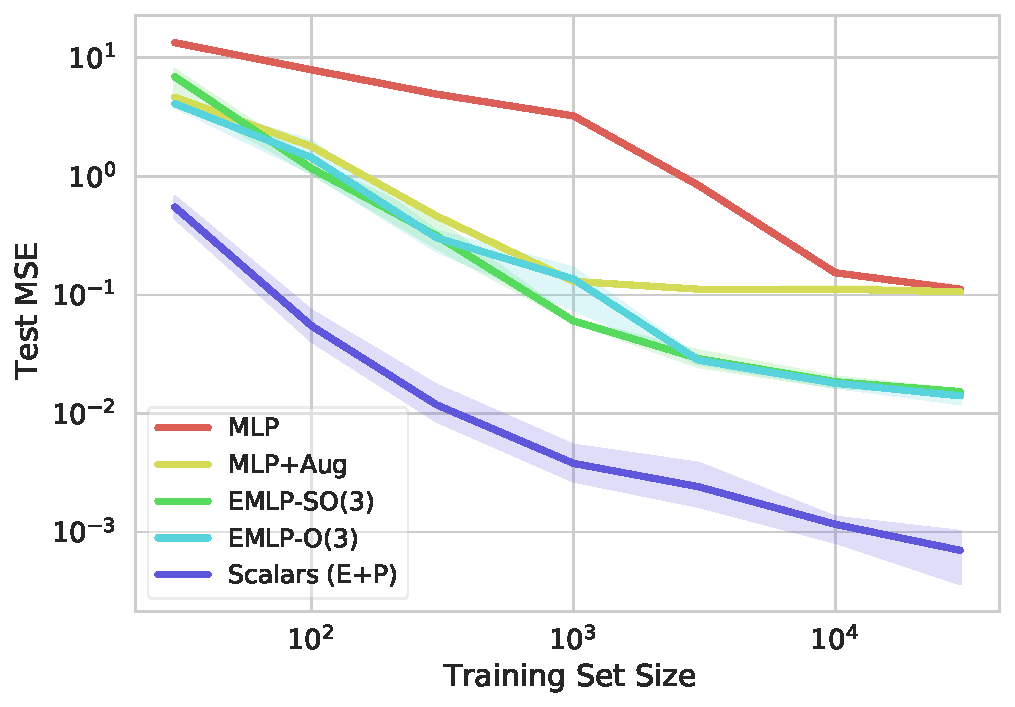
\includegraphics[scale=0.45]{data_efficiency_Inertia.pdf}
   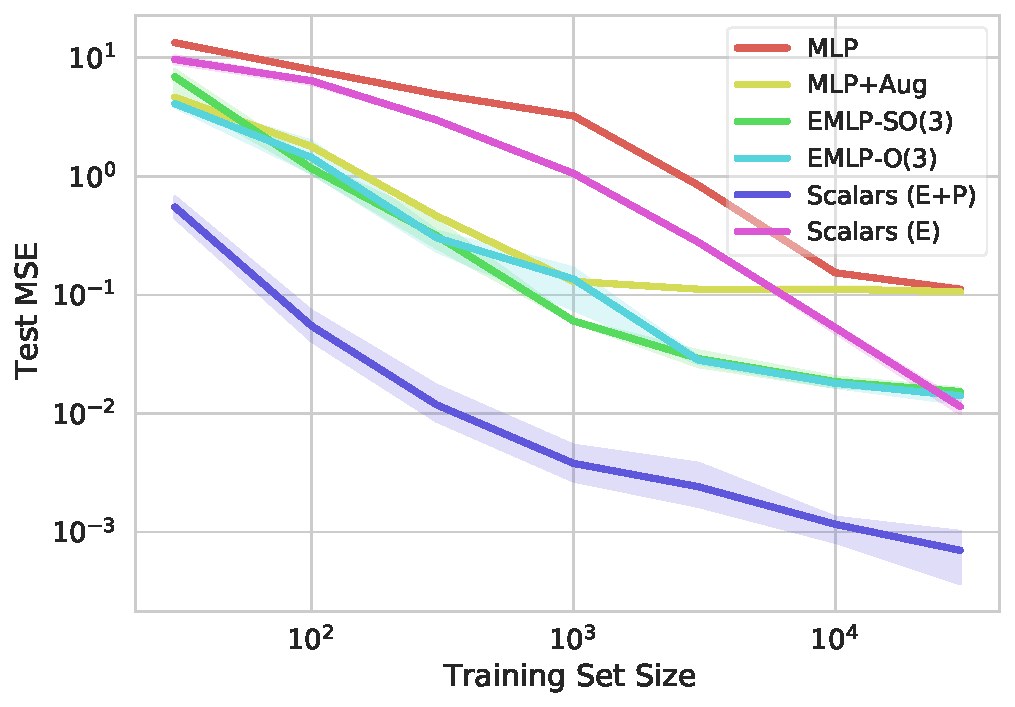
\includegraphics[scale=0.45]{data_efficiency_Inertia_noperm.pdf}
   \caption{O(3) equivariant task. All perceptrons used in \texttt{Scalars (E$+$P)} and \texttt{Scalars (E)} are with 2 layers and 200 hidden nodes. }
   \label{fig:O3equivariant}
\end{figure}

\end{document}